\documentclass{article}
\usepackage[utf8]{inputenc}
\usepackage{fullpage}
\usepackage{verbatim}
\usepackage{graphicx}
\usepackage{float}

\title{RabbitMQ}
\author{Rohit Singh}
\date{June 19th - 25th, 2022}

\begin{document}

\maketitle

\tableofcontents

\section{Overview}

\subsection{What is RabbitMQ?}

RabbitMQ is a messaging broker which acts as an intermediary for messaging. RabbitMQ gives applications a common platform to send and receive messages, as well as a location to store messages until the are received.

\subsection{RabbitMQ Features}

\subsubsection{Reliability}

RabbitMQ allows applications to trade off performance with reliability. The reliability features that RabbitMQ allows for as persistence, delivery acknowledgements, publisher confirms and high availability.

\subsubsection{Flexible Routing}

RabbitMQ features built-in exchange types for typical routing logic. These exchanges can be combined together to create more complex routing mechanisms.

\subsubsection{Clustering}

Multiple RabbitMQ servers on a local network can be clustered together to form a single logical broker.

\subsubsection{Federation}
RabbitMQ offers a federation model to allow servers to be configured as loosely or unreliably as needed, even if clustered with other servers.

\subsubsection{Highly Available Queues}

RabbitMQ supports data structures like \textbf{replicated queues} and \textbf{streams}. With these structures, if there is a hardware failure, messages are safe as long as the majority of cluster nodes are online.

\subsubsection{Multi-Protocol}

RabbitMQ supports messaging over a variety of protocols, such as:

\begin{itemize}
    \item MQTT
    \item HTTP and WebSockets
    \item AMQP 1.0
\end{itemize}

\subsubsection{Software Clients}

There are RabbitMQ clients for almost any language that you can think of

\subsubsection{Management UI}

RabbitMQ ships with an easy-to use UI, allowing for simple monitoring and controlling of every aspect of the message broker.

\subsubsection{Tracing}

If the system is misbehaving, RabbitMQ offers tracing support for easier debugging.

\subsubsection{Plugin System}

RabbitMQ has numerous plugins that can be used to extend it in different ways. 
Custom plugins can also be created for more specific use cases.

\subsection{Dictionary}

\subsubsection{Producing}

\textbf{Producing} means nothing more than sending.

A program that sends messages is a \textbf{producer}

\subsubsection{Queue}

A \textbf{queue} is the name for a post box which lives inside RabbitMQ.

Although messages flow through RabbitMQ and applications, they are only stored in a \textit{queue}, which is bound by the host's memory and disk limits. 

Many \textit{producers} can send messages that go to one queue, and many \textit{consumers} can try to receive data from one \textit{queue}.

\subsubsection{Consuming}

\textit{Consuming} is the same as receiving. A \textit{consumer} is a program that mostly waits to receive messages.

\section{Tutorials}

\subsection{Hello World!}

\textit{Source code located at}: \verb|the-big-repository-of-knowledge/RabbitMQ/tutorials/hello_world/|

\subsubsection{Introduction}

In this example, we are writing two programs in Python programs, one to act as the producer and another to act as a consumer. The producer will send a single message to the consumer which will print it out upon receiving it. 

The overall design will look like: 

\begin{figure}[H]
    \centering
    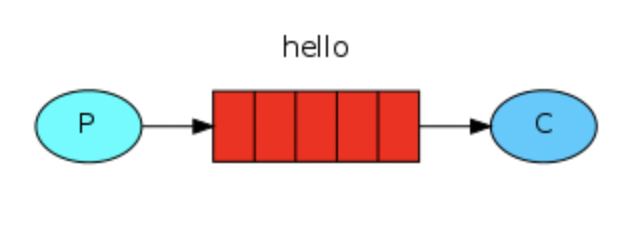
\includegraphics[scale=0.8]{RabbitMQ/images/t1-1.png}
    \caption{System Diagram (from https://www.rabbitmq.com/tutorials/tutorial-one-python.html)}
    \label{t1-1}
\end{figure}




\end{document}